\documentclass{standalone}
\standaloneconfig{border=10pt}
\usepackage[utf8]{inputenc}
\usepackage[french]{babel}
\usepackage{amsmath}
\usepackage{cases}
\usepackage{graphicx}
\usepackage{booktabs}

\begin{document}

\begin{minipage}{3in}
\setlength{\parindent}{10pt}
\setlength{\parskip}{3ex plus 0.5ex minus 0.2ex}

\textbf{\underline{Unité Arithématique et Logique (UAL)}}\\

\begin{figure}
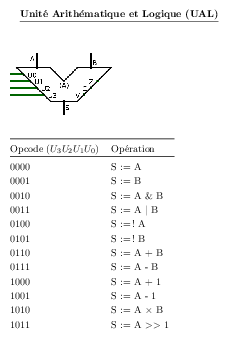
\includegraphics[width=0.5\textwidth]{ual.png}
\end{figure}
\renewcommand{\arraystretch}{1.2}
\begin{tabular}{@{}lllll@{}}
\toprule
 Opcode ($U_3U_2U_1U_0$) & Opération \\
\toprule
0000 & S := A \\
0001 & S := B \\
0010 & S := A \& B\\
0011 & S := A $\mid$ B\\
0100 & S := ! A\\
0101 & S := ! B\\
0110 & S := A + B\\
0111 & S := A - B\\
1000 & S := A + 1\\
1001 & S := A - 1\\
1010 & S := A $\times$ B\\
1011 & S := A $>>$ 1\\
\end{tabular}

\end{minipage}


\end{document}
